
\chapter{Thực nghiệm}
Mục tiêu thử nghiệm là minh họa sự so sánh giữa phương pháp được đề xuất bởi D-wave với phương pháp cải tiến của chúng ta nhằm xây dựng lại bài toán xếp hậu dựa trên mô hình bậc hai nhị phân.
\section{Cài đặt}
\subsection{Hệ thống}
Tất cả các thí nghiệm ủ lượng tử đều được thực hiện trên D-Wave Advantage, công cụ ủ lượng tử mới nhất do D-Wave System Inc trình bày. Phiên bản được sử dụng là Advantage System 4.1, tính toán lượng tử đoạn nhiệt dựa trên kiến trúc Pegasus với 5627 hạt lượng tử hoạt động. \cite{Performance Update} 
\subsection{Phương pháp}
Chúng ta sẽ chạy thử nghiệm so sánh các phương pháp sử dụng mô hình bậc hai nhị phân được thảo luận ở trên  bao gồm công thức bình phương do D-Wave đề xuất và công thức cộng dồn là công thức cải tiến của chúng ta.
%	\section{Parameters}

\subsection{Số liệu} 

Đối với mỗi công thức, chúng ta ghi lại số lượng biến ($\#Var$), số tương tác giữa các biến trong công thức QUBO($\#Interaction$), số lượng hạt lượng tử vật lý($\#Qubit$), tỷ lệ phần trăm các trường hợp trong đó một lời giải tối ưu được tìm thấy ($\%Sol$). 

$\%OptGap$ là khoảng cách từ lời giải tốt nhất tìm được tới lời giải tối ưu:
\[
	\%OptGap = \frac{n - n_{best}}{n}
\]
trong đó: n là số hậu cần đặt, $n_{best}$ là số hậu tốt nhất trong $\alpha$ lần chạy.

$TTS(t_f)$ là thời gian tìm ra được một lời giải với xác suất kỳ vọng là $N_{exp}$:

$$TTS(t_f) = t_f \cdot N_{exp}$$

trong đó: 
 $t_f$ là thời gian chạy trung bình của một lần đọc có tính đến thời gian lập trình ban đầu ($t_{prog}$), thời gian ủ ($t_{annealing}$) và thời gian đọc ( $t_{readout}$) cho mỗi mẫu:
		
		$$t_f = \frac{t_{prog}}{N_{read}} + t_{annealing} + t_{readout}$$
, $N_{exp}$ là xác suất kỳ vọng:
$$N_{exp} = \frac{1}{\%Sol}$$
Do đó, nó không bao gồm thời gian truy cập và thời gian nhúng QUBO vào biểu đồ phần cứng.

\section{Kết quả}

	\subsection{So sánh giữa các công thức }
	
	\begin{table}[H]
		\centering
		\begin{tabular}{ c c c c c c}
			\hline
			Công thức & \textbf{Bình phương} & \textbf{Cộng dồn} \\
			\hline
			\textbf{$\#Var$}     & $N^2$ & $3N^2 - 4N + 2$ \\
			\textbf{$\#Interaction$}     & $\frac{5}{3}N^3 - 2N^2 + \frac{N}{3}$ & $N^3 + 5N^2 -12N +6$\\
			
			\hline
		\end{tabular}
		\caption{Bảng công thức tính số lượng biến và số liên kết sử dụng trong công thức bình phương và công thức cộng dồn theo số quân hậu}
		\label{tab:var_and_interaction}
	\end{table}
	
		
	\begin{table}[H]
		\centering
		\begin{tabular}{|c|c|c|c|c|c|c|c|c|c|c|c|c|c|c|}
			\hline
			N & 4 & 5 & 6 & 7 & 8 & 9 & 10 & 11 & 12 & 13 & 14 & 15 & 16 \\
			\hline
			Bình phương & 16 & 25 & 36 & 49 & 64 & 81 & 100 & 121 & 144 & 169 & 196 & 225 & 256 \\
			\hline
			Cộng dồn & 34 & 57 & 86 & 121 & 162 & 209 & 262 & 321 & 386 & 457 & 534 & 617 & 706 \\
			\hline
		\end{tabular}
		
		
		
		\caption{Bảng số lượng biến sử dụng trong công thức bình phương và công thức cộng dồn theo số quân hậu}
		\label{tab:var_num}
	\end{table}
	
	\begin{figure}[H]
		\centering
		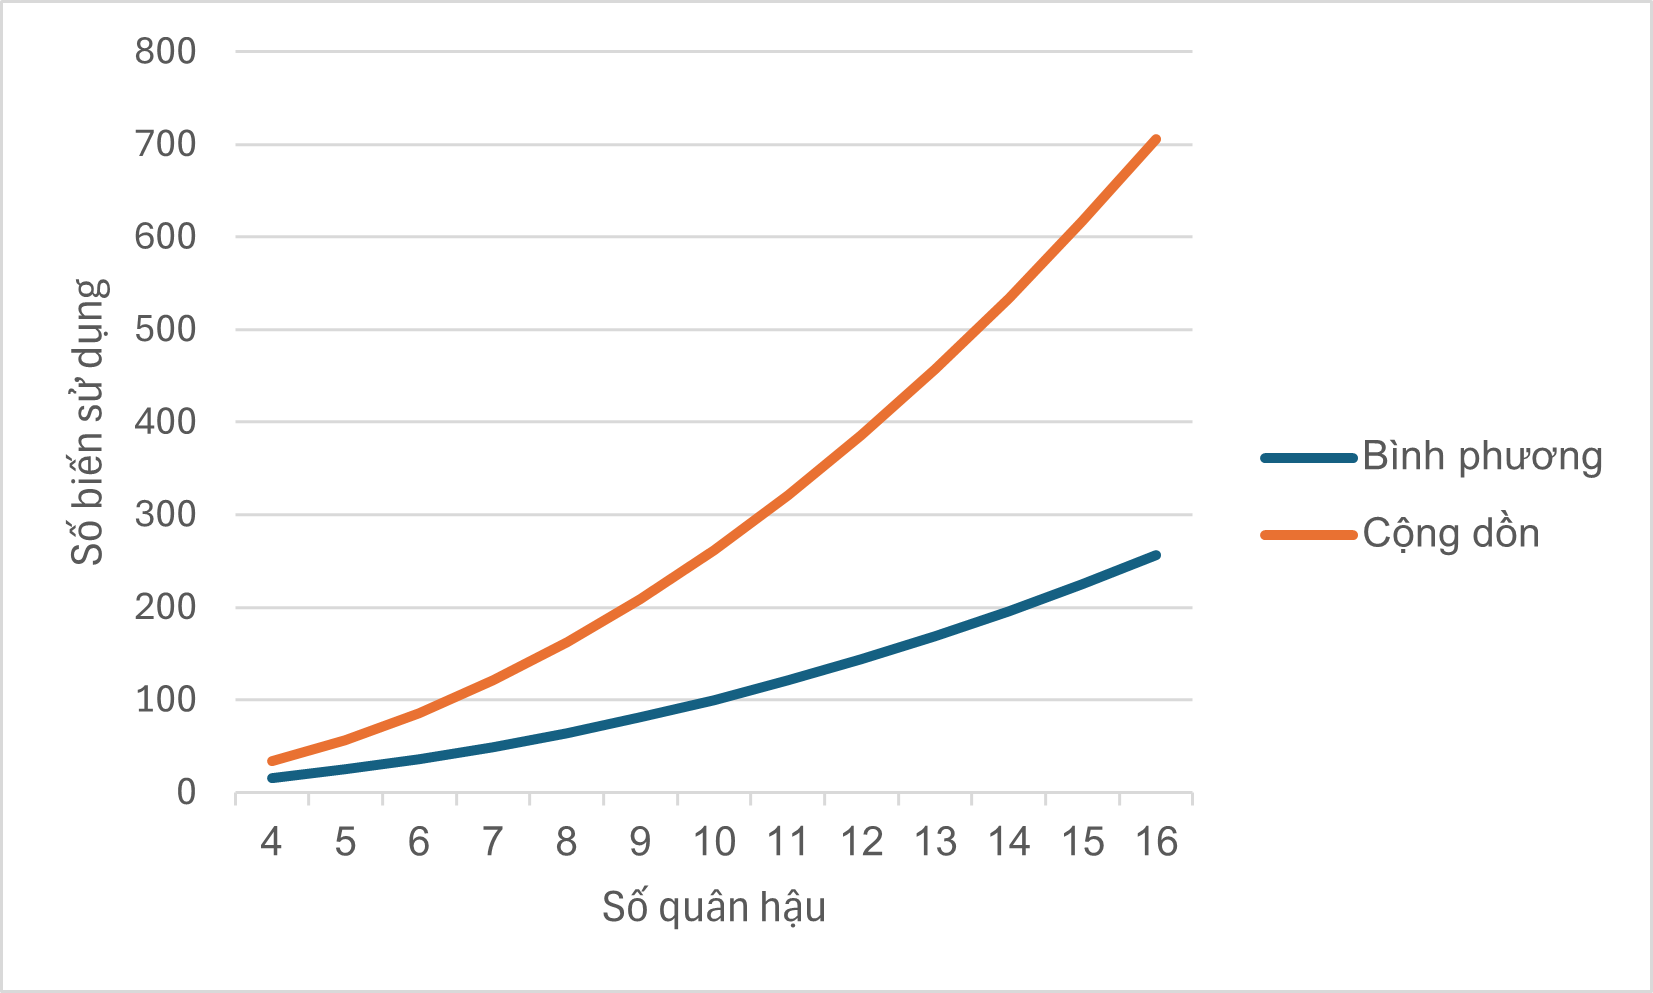
\includegraphics[width=0.7\textwidth]{images/methods/var_num.png}
		\caption{Biểu đồ số lượng biến sử dụng trong công thức bình phương và công thức cộng dồn theo số quân hậu}
		\label{fig:var_num}
	\end{figure}
	
	\begin{table}[H]
		\centering
		\begin{tabular}{|c|c|c|c|c|c|c|c|c|c|c|c|c|c|c|}
			\hline
			N & 4 & 5 & 6 & 7 & 8 & 9 & 10 & 11 & 12 & 13 & 14 & 15 & 16 \\
			\hline
			Bình phương & 76 & 160 & 290 & 476 & 728 & 1056 & 1470 & 1980 & 2596 & 3328 & 4186 & 5180 & 6320 \\
			\hline
			Cộng dồn & 102 & 196 & 330 & 510 & 742 & 1032 & 1386 & 1810 & 2310 & 2892 & 3562 & 4326 & 5190 \\
			\hline
		\end{tabular}
		
		
		
		\caption{Bảng số lượng tương tác giữa các biến trong công thức bình phương và công thức cộng dồn theo số quân hậu}
		\label{tab:interaction_num_cmp}
	\end{table}
	
	\begin{figure}[H]
		\centering
		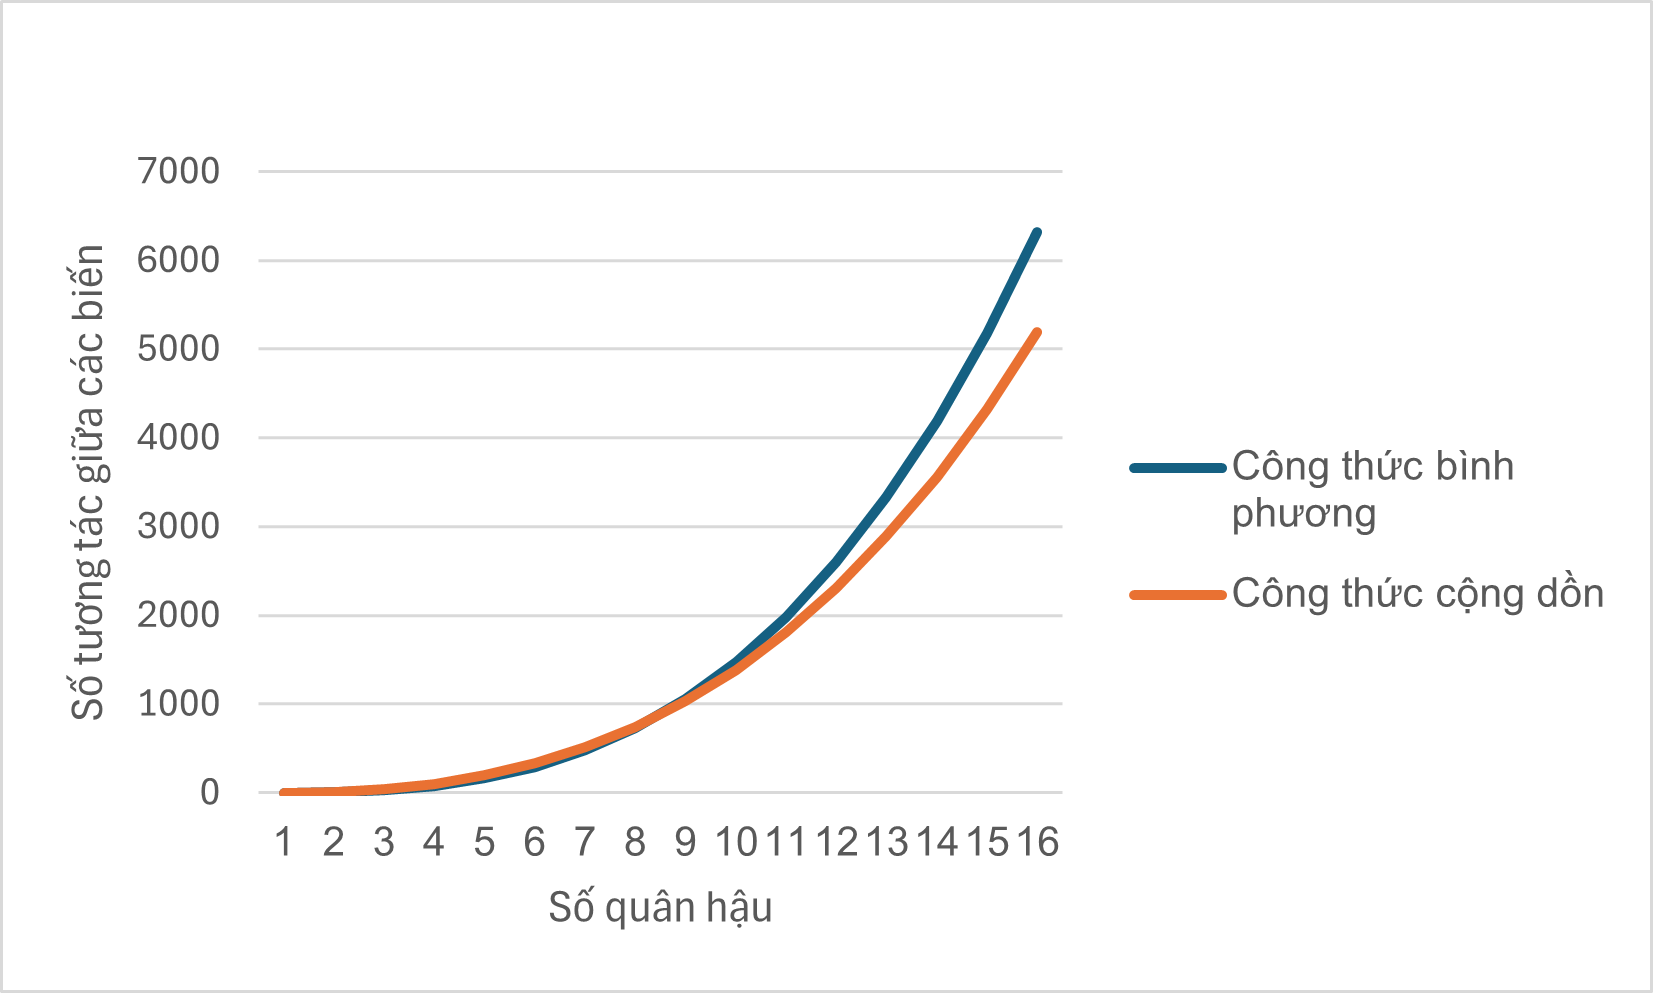
\includegraphics[width=0.7\textwidth]{images/interaction_num_cmp.png}
		\caption{Biểu đồ số lượng tương tác giữa các biến trong công thức bình phương và công thức cộng dồn theo số quân hậu }
		\label{fig:interaction_num_cmp}
	\end{figure}
	Như được hiển thị trong hình~\ref{fig:var_num}, do công thức cộng dồn cần sử dụng thêm biến phụ nên dễ dàng nhận thấy số lượng biến cần dùng của công thức bình phương luôn luôn ít hơn của công thức cộng dồn. Tuy nhiên, từ hình~\ref{fig:interaction_num_cmp} có thể thấy ban đầu số lượng liên kết công thức cộng dồn sử dụng vẫn nhỉnh hơn chút với đầu vào số quân hậu nhỏ, nhưng khi số quân hậu dần tăng lên thì công thức cộng dồn lại chiếm ưu thế so với công thức bình phương.


\begin{table}[H]
	\centering
	\begin{tabular}{|c|c|c|c|c|c|c|c|c|c|c|}
		\hline
		N & 4 & 5 & 6 & 7 & 8 & 9 & 10 & 11 & 12 & 13 \\
		\hline
		Bình phương & 32.{6} & 73 & 146.{3} & 264.{3} & 450.{6} & 759.{3} & 1187.{3} & 1708 & 2540.{3} & 3558.{6} \\
		\hline
		Cộng dồn & 63.{3} & 135 & 244 & 446.{3} & 704.{6} & 1086 & 1723.{3} & 2535 & 3249.{3} & 4167.{3} \\
		\hline
	\end{tabular}
	\caption{Bảng số lượng hạt lượng tử vật lý cần dùng trong công thức bình phương và công thức cộng dồn theo số quân hậu}
	\label{tab:num_qubit}
\end{table}

\begin{figure}[H]
	\centering
	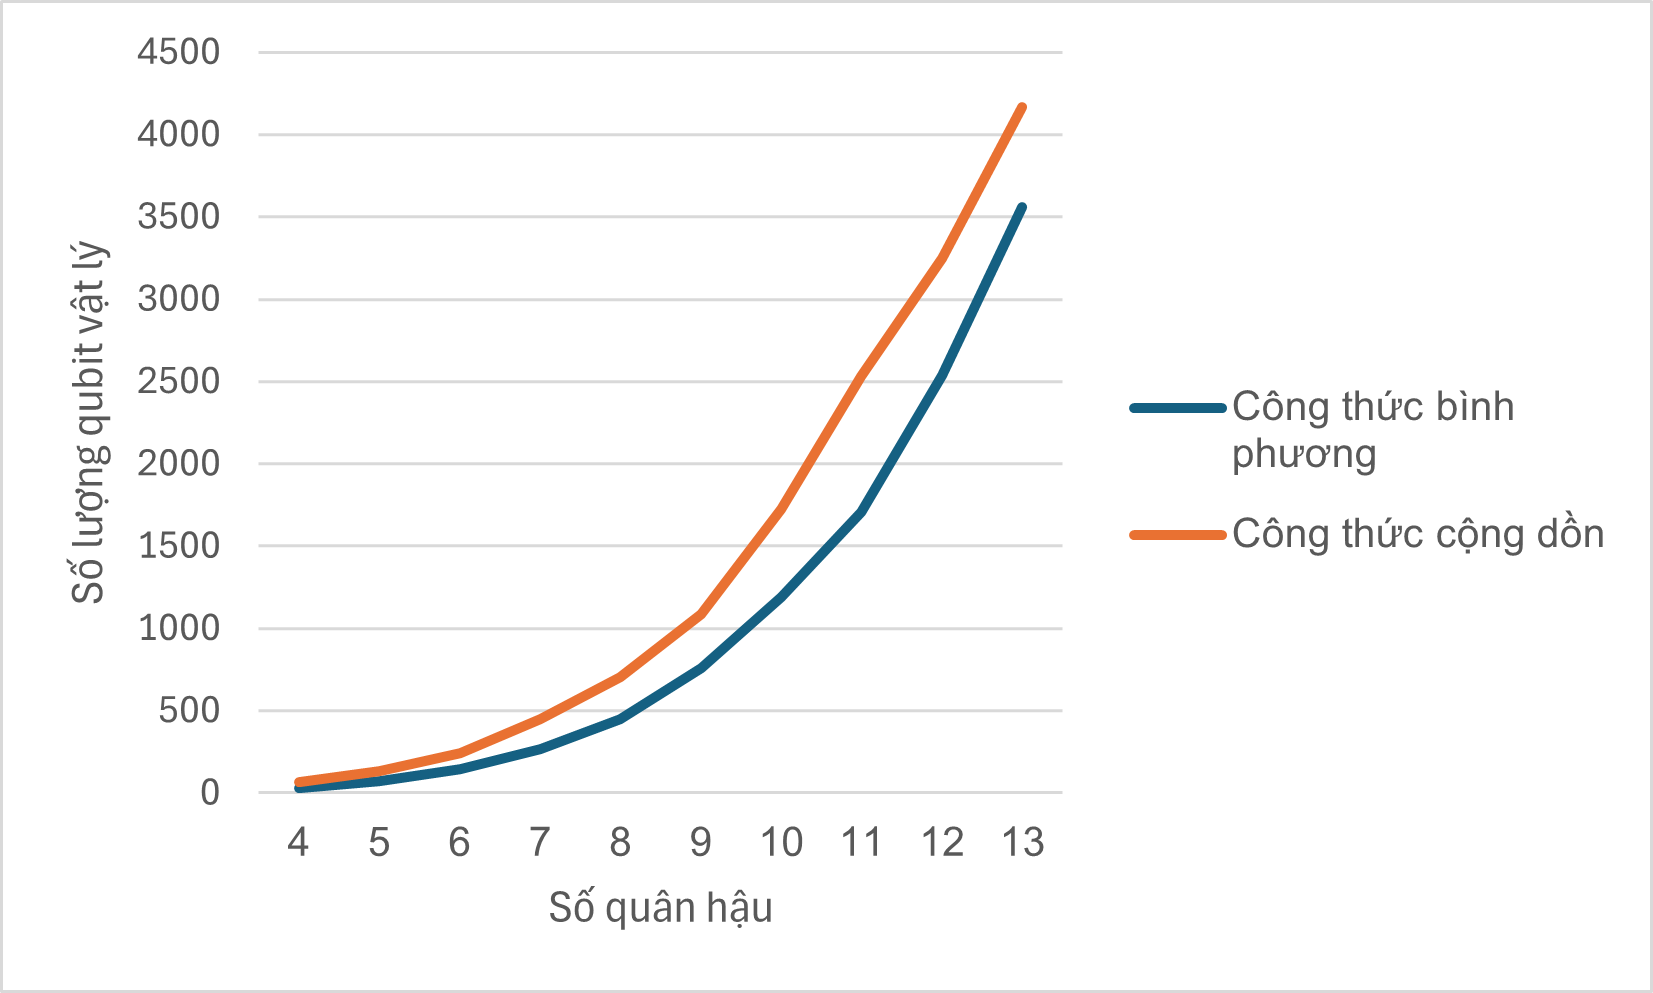
\includegraphics[width=0.7\textwidth]{images/methods/num_qubit.png}
	\caption{Biểu đồ số lượng hạt lượng tử vật lý cần dùng trong công thức bình phương và công thức cộng dồn theo số quân hậu}
	\label{fig:num_qubit}
\end{figure}


\begin{table}[H]
	\centering
	\begin{tabular}{|c|c|c|c|c|c|c|c|c|c|c|}
		\hline
		N & 4 & 5 & 6 & 7 & 8 & 9 & 10 & 11 & 12 & 13 \\
		\hline
		Bình phương & 85.53 & 58.1 & 4.6 & 2.8 & 0 & 0 & 0 & 0 & 0 & 0 \\
		\hline
		Cộng dồn & 25.63 & 10.43 & 0.07 & 0.03 & 0 & 0 & 0 & 0 & 0 & 0 \\
		\hline
	\end{tabular}
	
	\caption{Bảng tỷ lệ phần trăm lời giải tối ưu được tìm thấy ($\%sol$) trong công thức bình phương và công thức cộng dồn theo số quân hậu}
	\label{tab:methods/sol}
\end{table}

\begin{figure}[H]
	\centering
	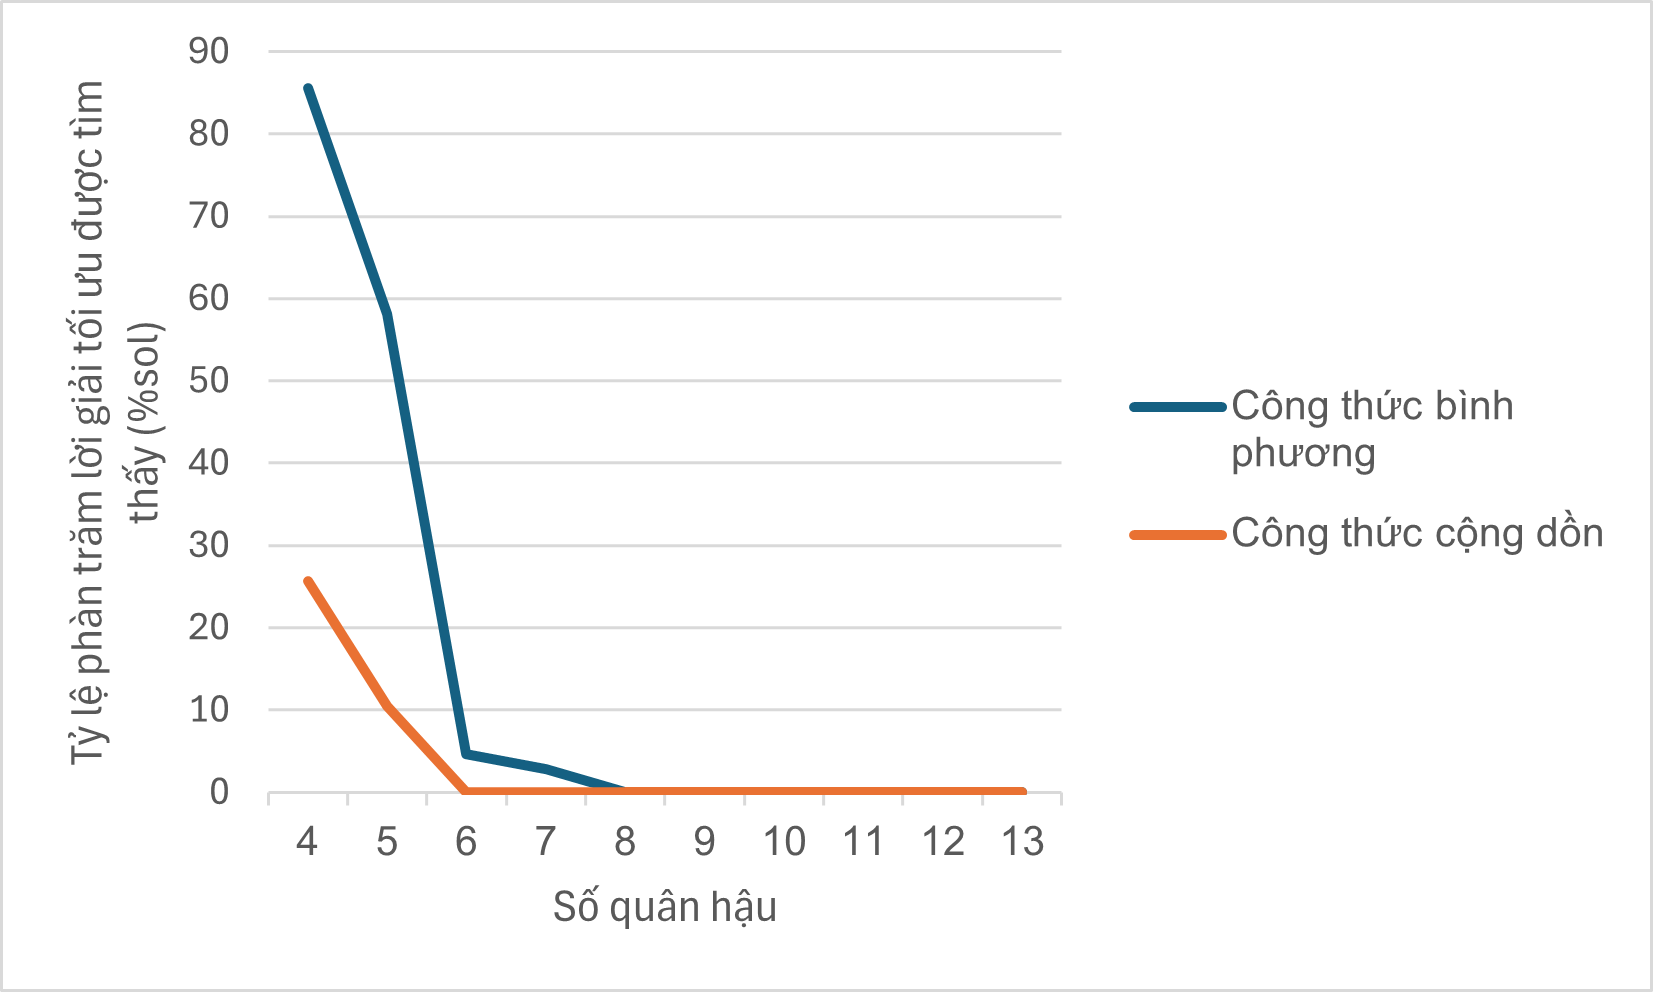
\includegraphics[width=0.7\textwidth]{images/methods/sol.png}
	\caption{Biểu đồ tỷ lệ phần trăm lời giải tối ưu tìm được ($\%sol$) trong công thức bình phương và công thức cộng dồn theo số quân hậu}
	\label{fig:methods/sol}
\end{figure}

Tuy công thức cộng dồn làm giảm bớt số liên kết giữa các biến nhưng việc tăng số lượng biến vẫn cho thấy số lượng hạt lượng tử cần dùng không những không giảm mà còn cần dùng nhiều hơn (Hình~\ref{fig:num_qubit}). Thêm vào đó, tỷ lệ phần trăm lời giải tối ưu được tìm thấy cũng giảm theo (Hình~\ref{fig:methods/sol}).

\begin{table}[H]
	\centering
	\begin{tabular}{|c|c|c|c|c|c|c|c|c|c|c|}
		\hline
		N & 4 & 5 & 6 & 7 & 8 & 9 & 10 & 11 & 12 & 13 \\
		\hline
		Bình phương & 0 & 0 & 0 & 0 & 4.16 & 7.41 & 20 & 18.18 & 22.22 & 25.64 \\
		\hline
		Cộng dồn & 0 & 0 & 0 & 0 & 4.17 & 14.81 & 6.67 & 18.18 & 30.55 & 25.64 \\
		\hline
	\end{tabular}
	
	
	\caption{Bảng khoảng cách từ lời giải tốt nhất tìm được tới lời giải tối ưu ($\%OptGap$) trong công thức bình phương và công thức cộng dồn theo số quân hậu}
	\label{tab:methods/optgap}
\end{table}

\begin{figure}[H]
	\centering
	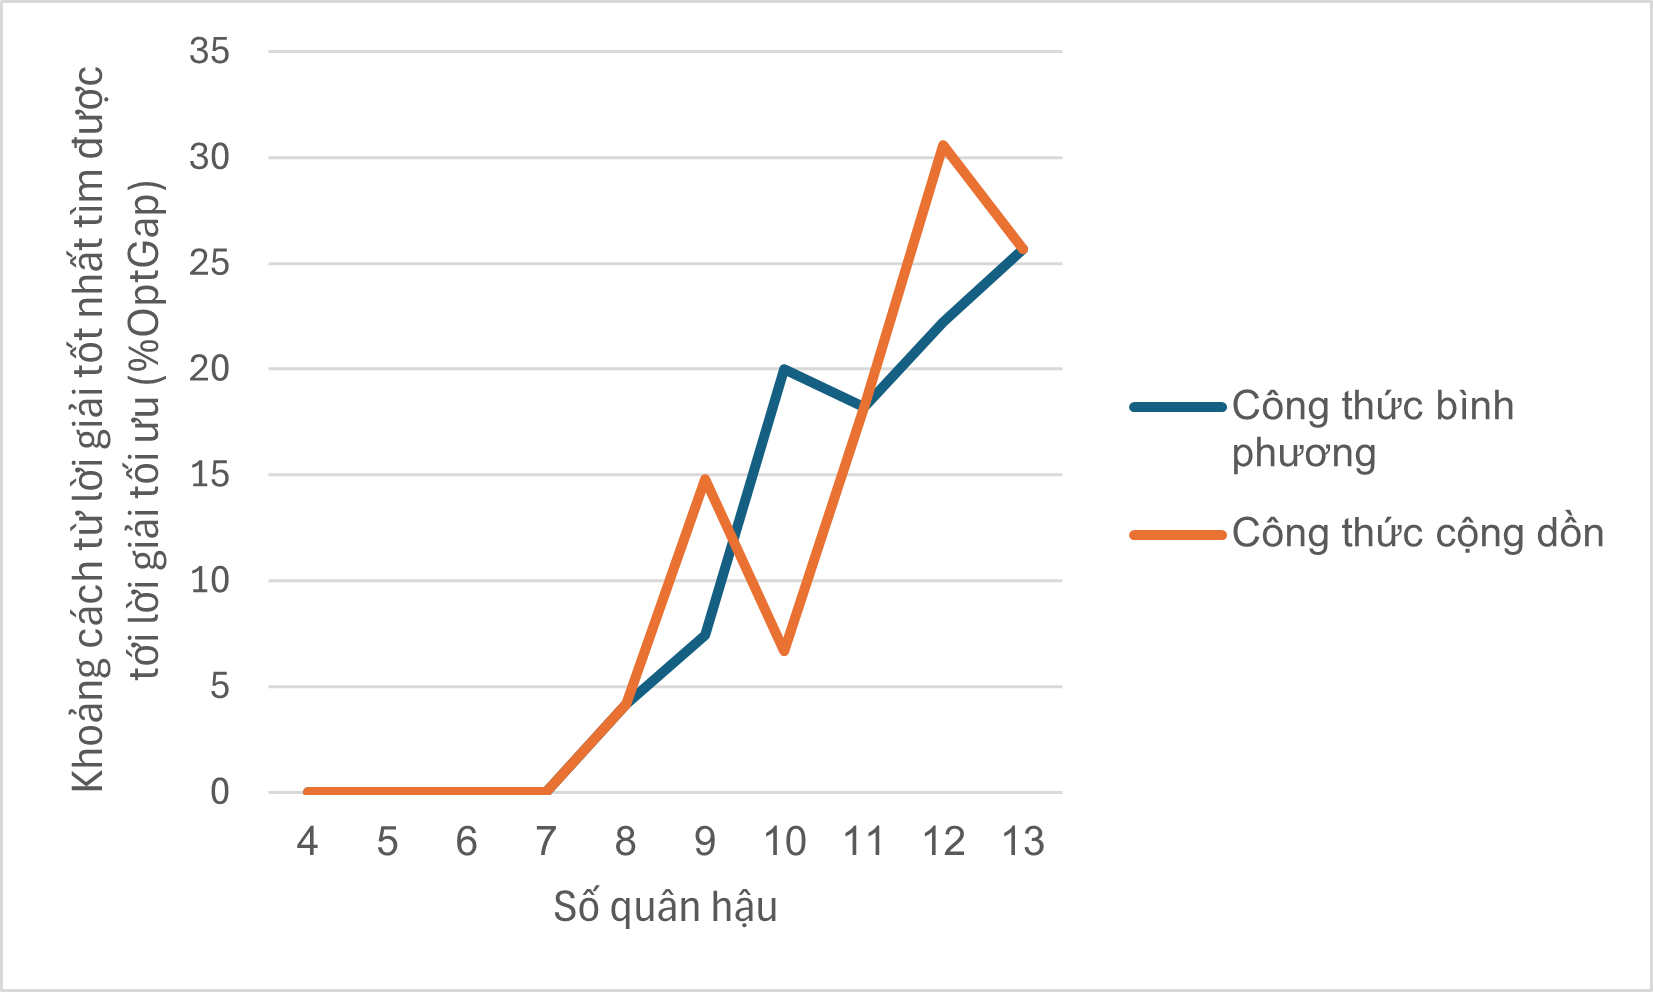
\includegraphics[width=0.7\textwidth]{images/methods/optgap.png}
	\caption{Biểu đồ khoảng cách từ lời giải tốt nhất tìm được tới lời giải tối ưu ($\%OptGap$) trong công thức bình phương và công thức cộng dồn theo số quân hậu}
	\label{fig:methods/optgap}
\end{figure}

Với điều kiện tiên quyết là giảm bớt số liên kết và chỉ cần lời giải gần đúng thì hình~\ref{fig:methods/optgap} cho thấy công thức cộng dồn vẫn coi là chấp nhận được, tuy rằng $\%OptGap$ có dao động đôi chút.

	\subsection{So sánh với ủ mô phỏng}
	
		\begin{table}[H]
		\centering
		\begin{tabular}{|c|c|c|c|c|c|c|c|c|c|c|}
			\hline
			N & 4 & 5 & 6 & 7 & 8 & 9 & 10 & 11 & 12 & 13 \\
			\hline
			Ủ lượng tử & 0.12 & 0.14 & 0.19 & 0.19 & 0.15 & 0.19 & 0.21 & 0.23 & 0.25 & 0.27 \\
			\hline
			Ủ mô phỏng & 0.23 & 0.39 & 0.58 & 0.81 & 1.05 & 1.37 & 1.78 & 2.24 & 2.76 & 3.3 \\
			\hline
		\end{tabular}
		
		
		\caption{Bảng thời gian chạy trung bình của một lần đọc (ms)  của ủ lượng tử và ủ mô phỏng theo số quân hậu}
		\label{tab:SA_QA/t_f}
	\end{table}
	
	\begin{figure}[H]
		\centering
		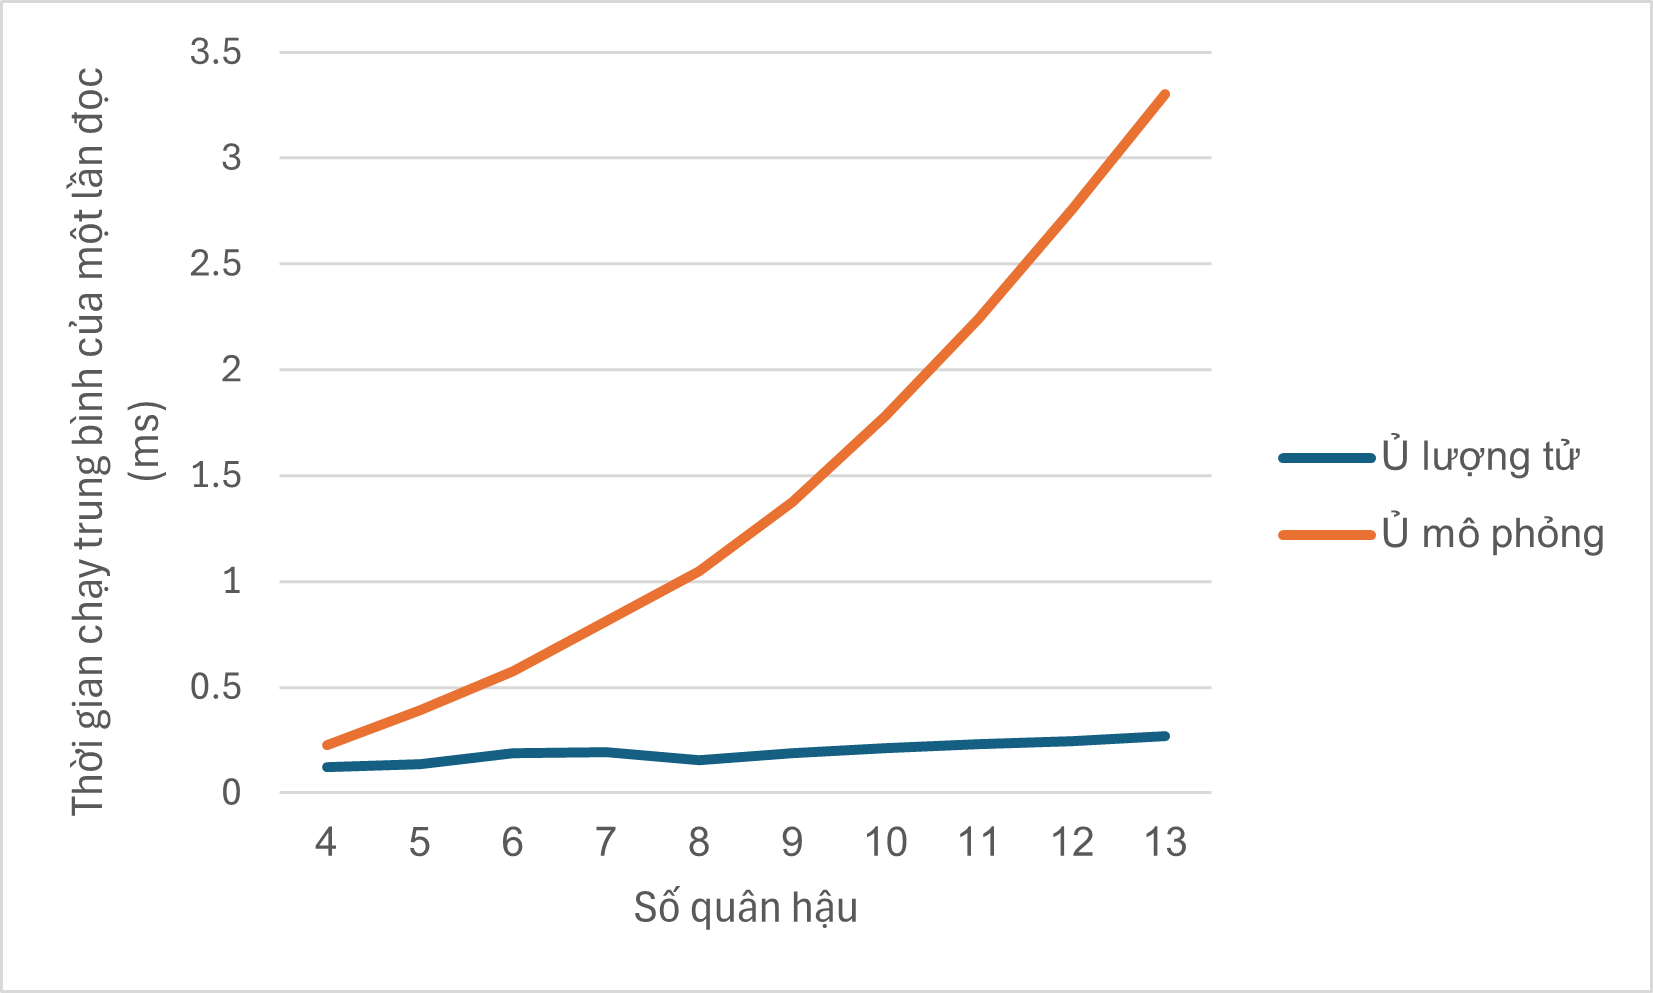
\includegraphics[width=0.7\textwidth]{images/SA_QA/t_f.png}
		\caption{Biểu đồ thời gian chạy trung bình của một lần đọc (ms)  của ủ lượng tử và ủ mô phỏng theo số quân hậu}
		\label{fig:SA_QA/t_f}
	\end{figure}
	Hình \ref{fig:SA_QA/t_f} đã chỉ ra độ phức tạp về thời gian có tác động lớn đối với quá trình ủ mô phỏng và nó không phải là hằng số. Ngược lại, quá trình ủ lượng tử thực sự có độ phức tạp về thời gian không đổi.
	
		\begin{table}[H]
		\centering
		\begin{tabular}{|c|c|c|c|c|c|c|c|c|c|c|}
			\hline
			N & 4 & 5 & 6 & 7 & 8 & 9 & 10 & 11 & 12 & 13 \\
			\hline
			Ủ lượng tử & 85.53 & 58.1 & 4.6 & 2.8 & 0 & 0 & 0 & 0 & 0 & 0 \\
			\hline
			Ủ mô phỏng & 100 & 100 & 97.6 & 98.93 & 99.67 & 99.7 & 99.47 & 99.4 & 99.67 & 99.67 \\
			\hline
		\end{tabular}
		
		
		\caption{Bảng tỷ lệ phần trăm lời giải tối ưu được tìm thấy ($\%sol$)  của ủ lượng tử và ủ mô phỏng theo số quân hậu}
		\label{tab:SA_QA/sol}
	\end{table}
	
	
	\begin{figure}[H]
		\centering
		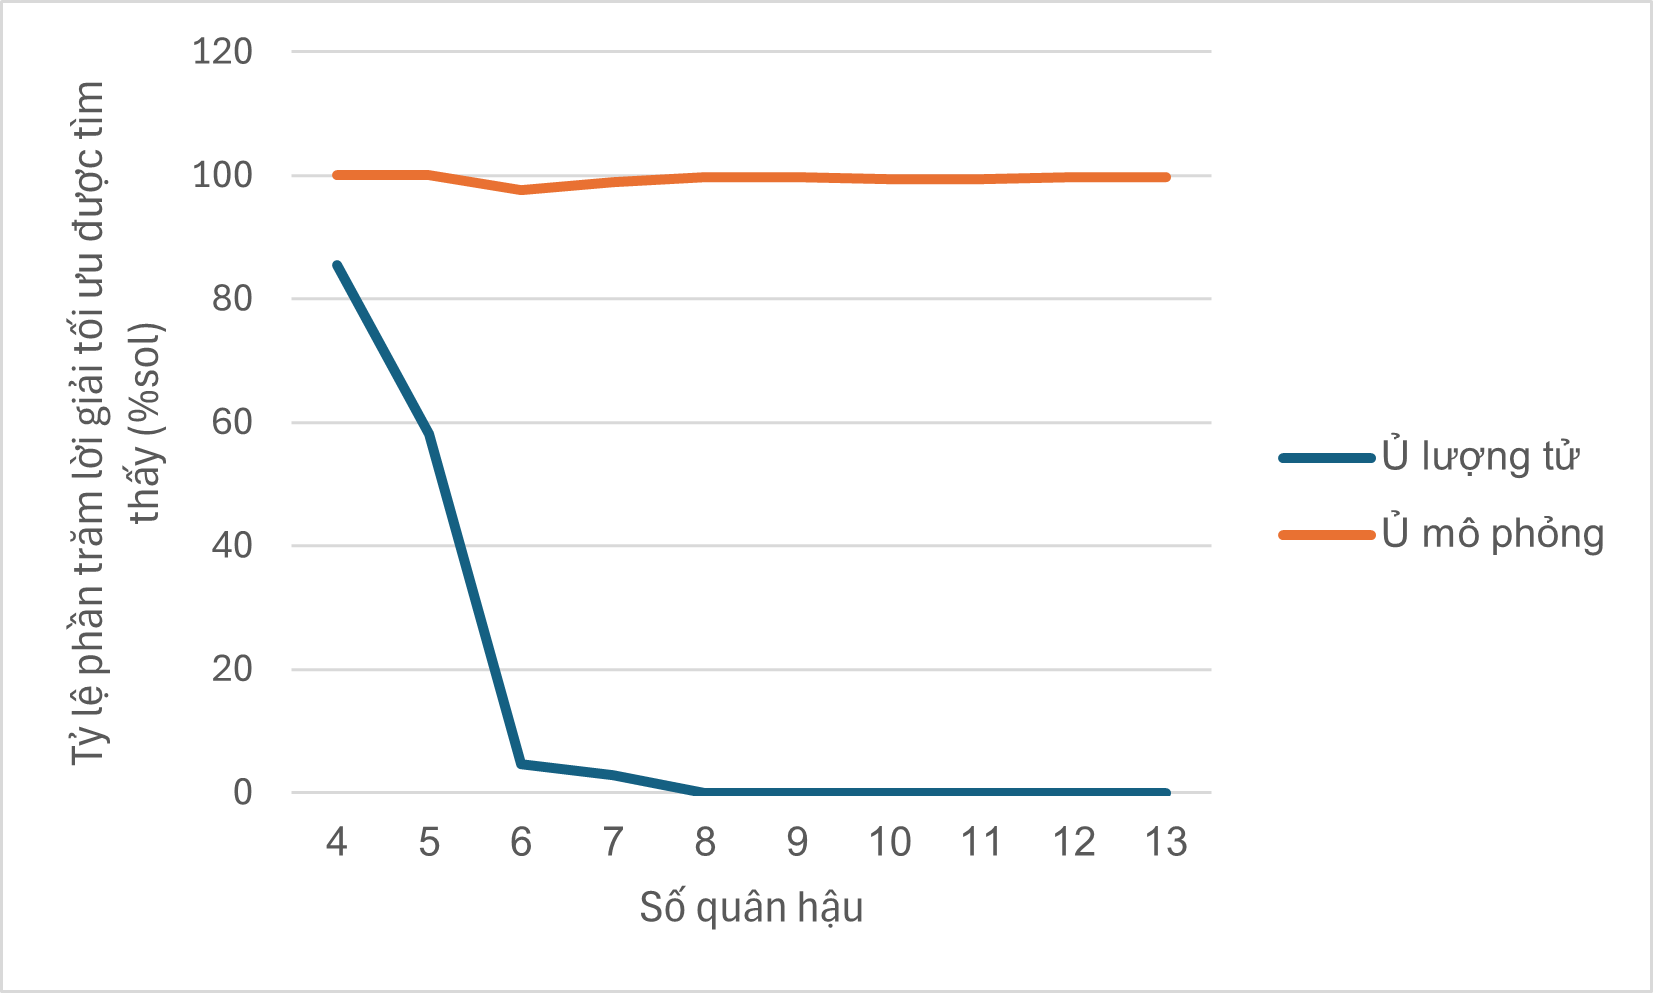
\includegraphics[width=0.7\textwidth]{images/SA_QA/sol.png}
		\caption{Biểu đồ tỷ lệ phần trăm lời giải tối ưu ($\%sol$)  của ủ lượng tử và ủ mô phỏng theo số quân hậu}
		\label{fig:SA_QA/sol}
	\end{figure}
	
	
	\begin{table}[H]
		\centering
		\begin{tabular}{|c|c|c|c|c|}
			\hline
			N & 4 & 5 & 6 & 7 \\
			\hline
			Ủ lượng tử & 0.1418 & 0.2358 & 4.1169 & 6.9181 \\
			\hline
			Ủ mô phỏng & 0.2284 & 0.3914 & 0.5899 & 0.8192 \\
			\hline
		\end{tabular}
		
		
		\caption{Bảng thời gian trung bình tìm ra một lời giải (ms)  của ủ lượng tử và ủ mô phỏng theo số quân hậu}
		\label{tab:SA_QA/TTS}
	\end{table}
	\begin{figure}[H]
		\centering
		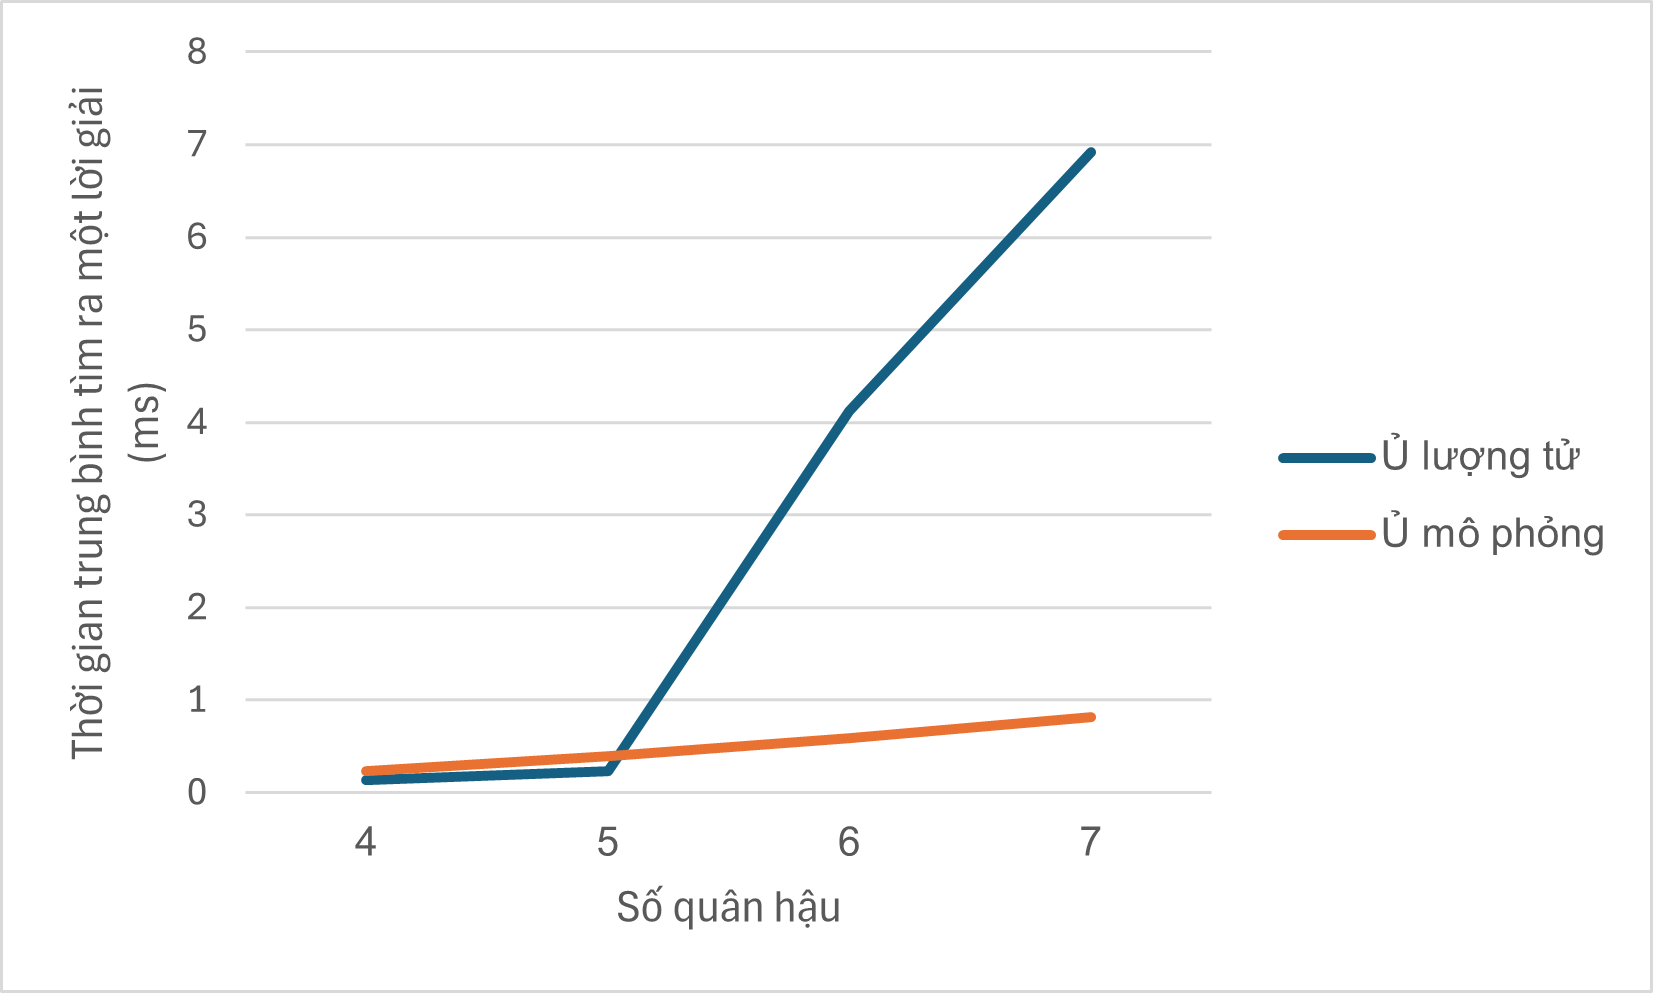
\includegraphics[width=0.7\textwidth]{images/SA_QA/TTS.png}
		\caption{Biểu đồ thời gian trung bình tìm ra một lời giải (ms)  của ủ lượng tử và ủ mô phỏng theo số quân hậu}
		\label{fig:SA_QA/TTS}
	\end{figure}
	
Như biểu diễn trong hình~\ref{fig:SA_QA/sol},~\ref{fig:SA_QA/TTS}, ủ lượng tử trong bài toán xếp hậu thực sự kém cạnh so với ủ mô phỏng cả về tỷ lệ lời giải tối ưu tìm thấy và thời gian tìm ra lời giải.
	